\chapter{Résultats et discussion}

\section{Données}
Dans ce chapitre, nous allons décrire les pré-traitement sur les données (images) et mentionner leur source ainsi que le mode d'accès.
\subsection{Source et nature de données}

\subsubsection{SDSS(Sloan Digital Sky Survey IV)}
En termes simples, le Sloan Digital Sky Survey est l'étude astronomique la plus ambitieuse jamais entreprise. SDSS a observé en détail un quart de l'ensemble du ciel, déterminant les positions et la luminosité absolue de centaines de millions d'objets célestes\cite{sdss}. Il mesure également les distances à plus d'un million de galaxies et quasars\footnote{http://skyserver.sdss.org/dr13/en/sdss/sdsshome.aspx}. 

\subsubsection{DR13 (database release version 13)} \footnote{http://skyserver.sdss.org/dr13/en/help/browser/browser.aspx}
Data Release 13 stocke les prèmieres données de la quatièmes phase de la collecte de SDSS. Elle inclut les données prises à partir de 25 juin 2015, and englobe plus que un tiers de la sphère céleste. Avec plusieurs mesures du ciel faites et dans plusieurs façons la taille de la base de données DR12 peut de plusieurs manières, 1231051050 objets (catalogues) ont été collectés \footnote{http://www.sdss.org/dr13/scope/} 

\begin{figure}[H]
    \centering
    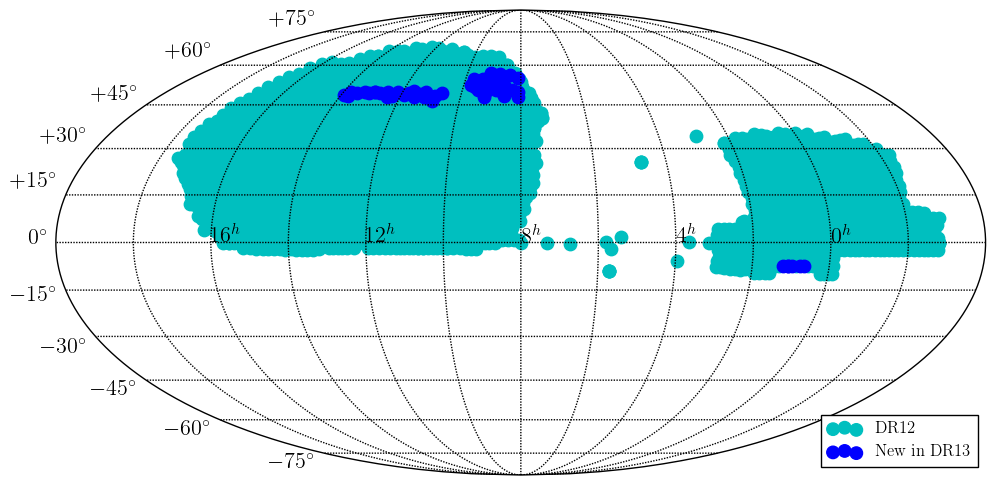
\includegraphics[scale = 0.5]{images/dr13_boss.png}
    %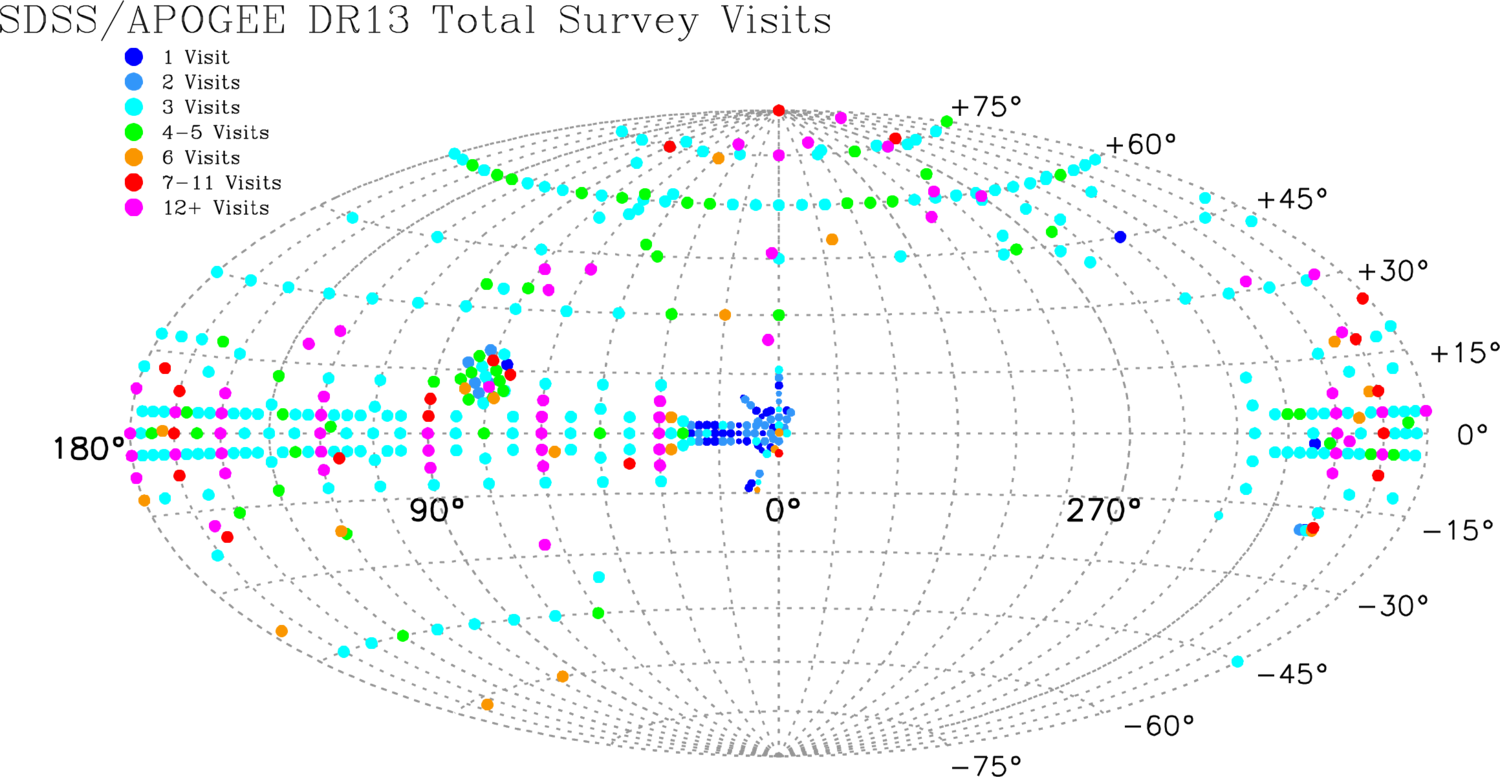
\includegraphics[scale = 0.3]{images/appoge.png}
    %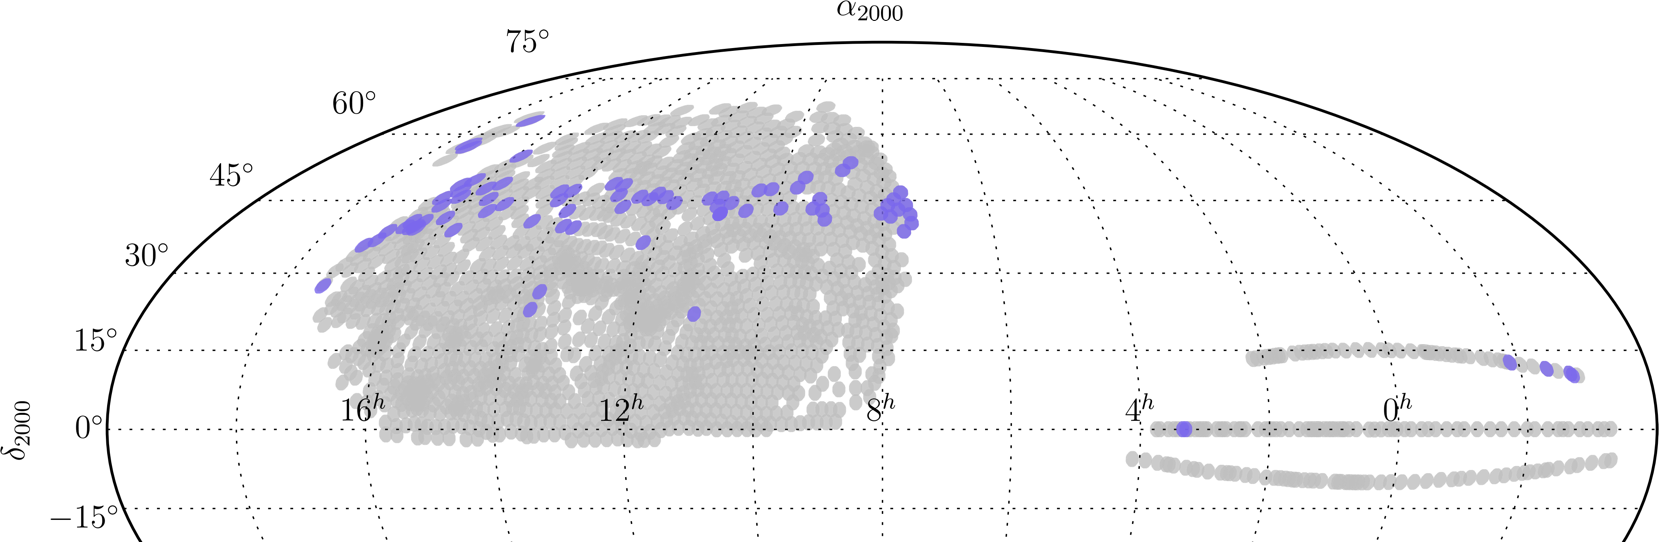
\includegraphics[scale = 0.1]{images/manga.png}
    \caption{eBOSS surveys}%, APOGEE surveys, and MaNGA surveys respectivement de gauche vers droite}
\end{figure}

Toutes nos données proviennent de la collecte de données SDSS . Elles sont télé-chargées sous forme des vecteurs chacune dans 5 bandes différentes (griuz). À partir de ces données sous forme de vecteurs provenant des tables SpecPhoto et PhotoPrimary de DR13 de SDSS, les urls des images correspondant à chaque vecteur sont générés. À partir de ces urls, les images sont télé-chargées et sauvegardées localement. 

\subsection{Pré-traitement sur les images}
Les images dans leur taille d'origine sont très grandes (1361*2048 pixels), et contiennent des quantités lumineuses très variées.
La taille de chaque image est réduite à 32*32, cette réduite est faite en utilisant les coordonnées centrales (rowc$\_$ et colc$\_$) des objets(images) dans chaque bande. Pour normaliser, le minimum de la quantité lumineuse (pixel) de chaque image est soustraite de l'image et le logarithme est appliqué à chaque pixel de l'image.  


\begin{figure}[H]
    \centering
    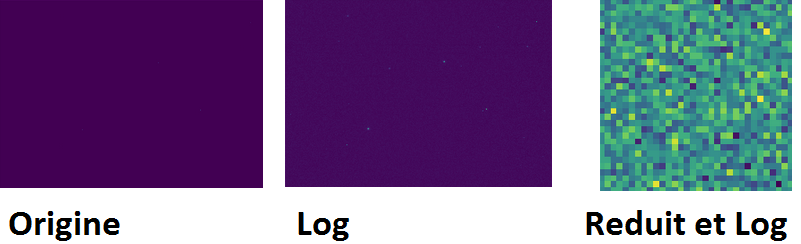
\includegraphics[scale = 0.5]{images/pretaitemen.png}
    \caption{pretement sur les images}
\end{figure}

\section{Configurations techniques}
Pendant toutes nos expérimentations, nous avons utilisés des machines hpc (haute performance computing) équipées de processeurs graphiques. Elles sont du type 

Pour la concrétisation de notre architecture du CNN, nous avons utilisé la bibliothèque Keras \cite{chollet2015keras}  et pour celle du boosting nous avons utilisé la bibliothèque skLearn \cite{scikit-learn}.
\section{Configuration des modèle}
Dans ce travail, nous avons choisi d'utiliser deux principales modèles de l'apprentissage automatique à savoir boosting qui est un modèle ensembliste, et réseau de neurones convolutifs (apprentissage profonds). En effets le boosting et les réseaux convolutifs ont donnée des bons résultats non pas seulement sur l'estimation du redshift \cite{meuphirim, isanto} mais également sur d'autres problèmes de régression et classification \cite{boost, adavencedCNN}. \\

Le choix et l'adaptation des hyper-paramètres ont été fait manuellement pour les deux types de modèles en faisant des test sur un petit échantillon de données et quelques combinaisons des hyper-paramètres. Au niveau du CNN, l'obtention des bons hyper-paramètres est compliquée car le CNN possède beaucoup d'hyper-paramètres à adapter.
\subsection{CNN (type: inception module)}
Notre modèle final, celui qui s'adapte bien à nos données c'est-à-dire qui réduit mieux l'erreur normalisée ($\Delta z_{norm}$) est un réseau convolutif de la famille des inceptions modules. 
\subsection{Boosting (type: xgboost)}
Trois principaux hyper-paramètres (nombre d'estimateurs, taux d'apprentissage et la profondeur de l'arbre) ont été réglés et adapté et tout le reste des paramètres ont été laissé avec leurs valeurs par défaut. Les trois modèles configurés du boosting sont mentionnés dans le tableau \ref{param_boost}.\\
\textbf{Quelques paramètres commun}
learning\_rate = 0.1, colsample\_bylevel=0.592, reg\_alpha=0.651, reg\_lambda=2.84, seed=5555
\begin{table}[H]
    \centering
    \begin{tabular}{|l|l|l|}
         \hline 
         modèles&n\_estimators&max\_depth\\
         \hline
          model1 &150&6\\
         \hline
         model3&150&5\\
         \hline         
         model2 &200&5\\
         \hline
         %mod1&&&&&&&
         %\hline
    \end{tabular}
    \caption{Paramètres de différents modèles de xgboost}
    \label{param_boost}
\end{table}

\section{Expérimentions avec CNN}
\section{Expérimentions avec XGBoost}
\section{Discussion}


















